\documentclass[tikz]{standalone}
\usetikzlibrary{calc, intersections, math}

\begin{document}
	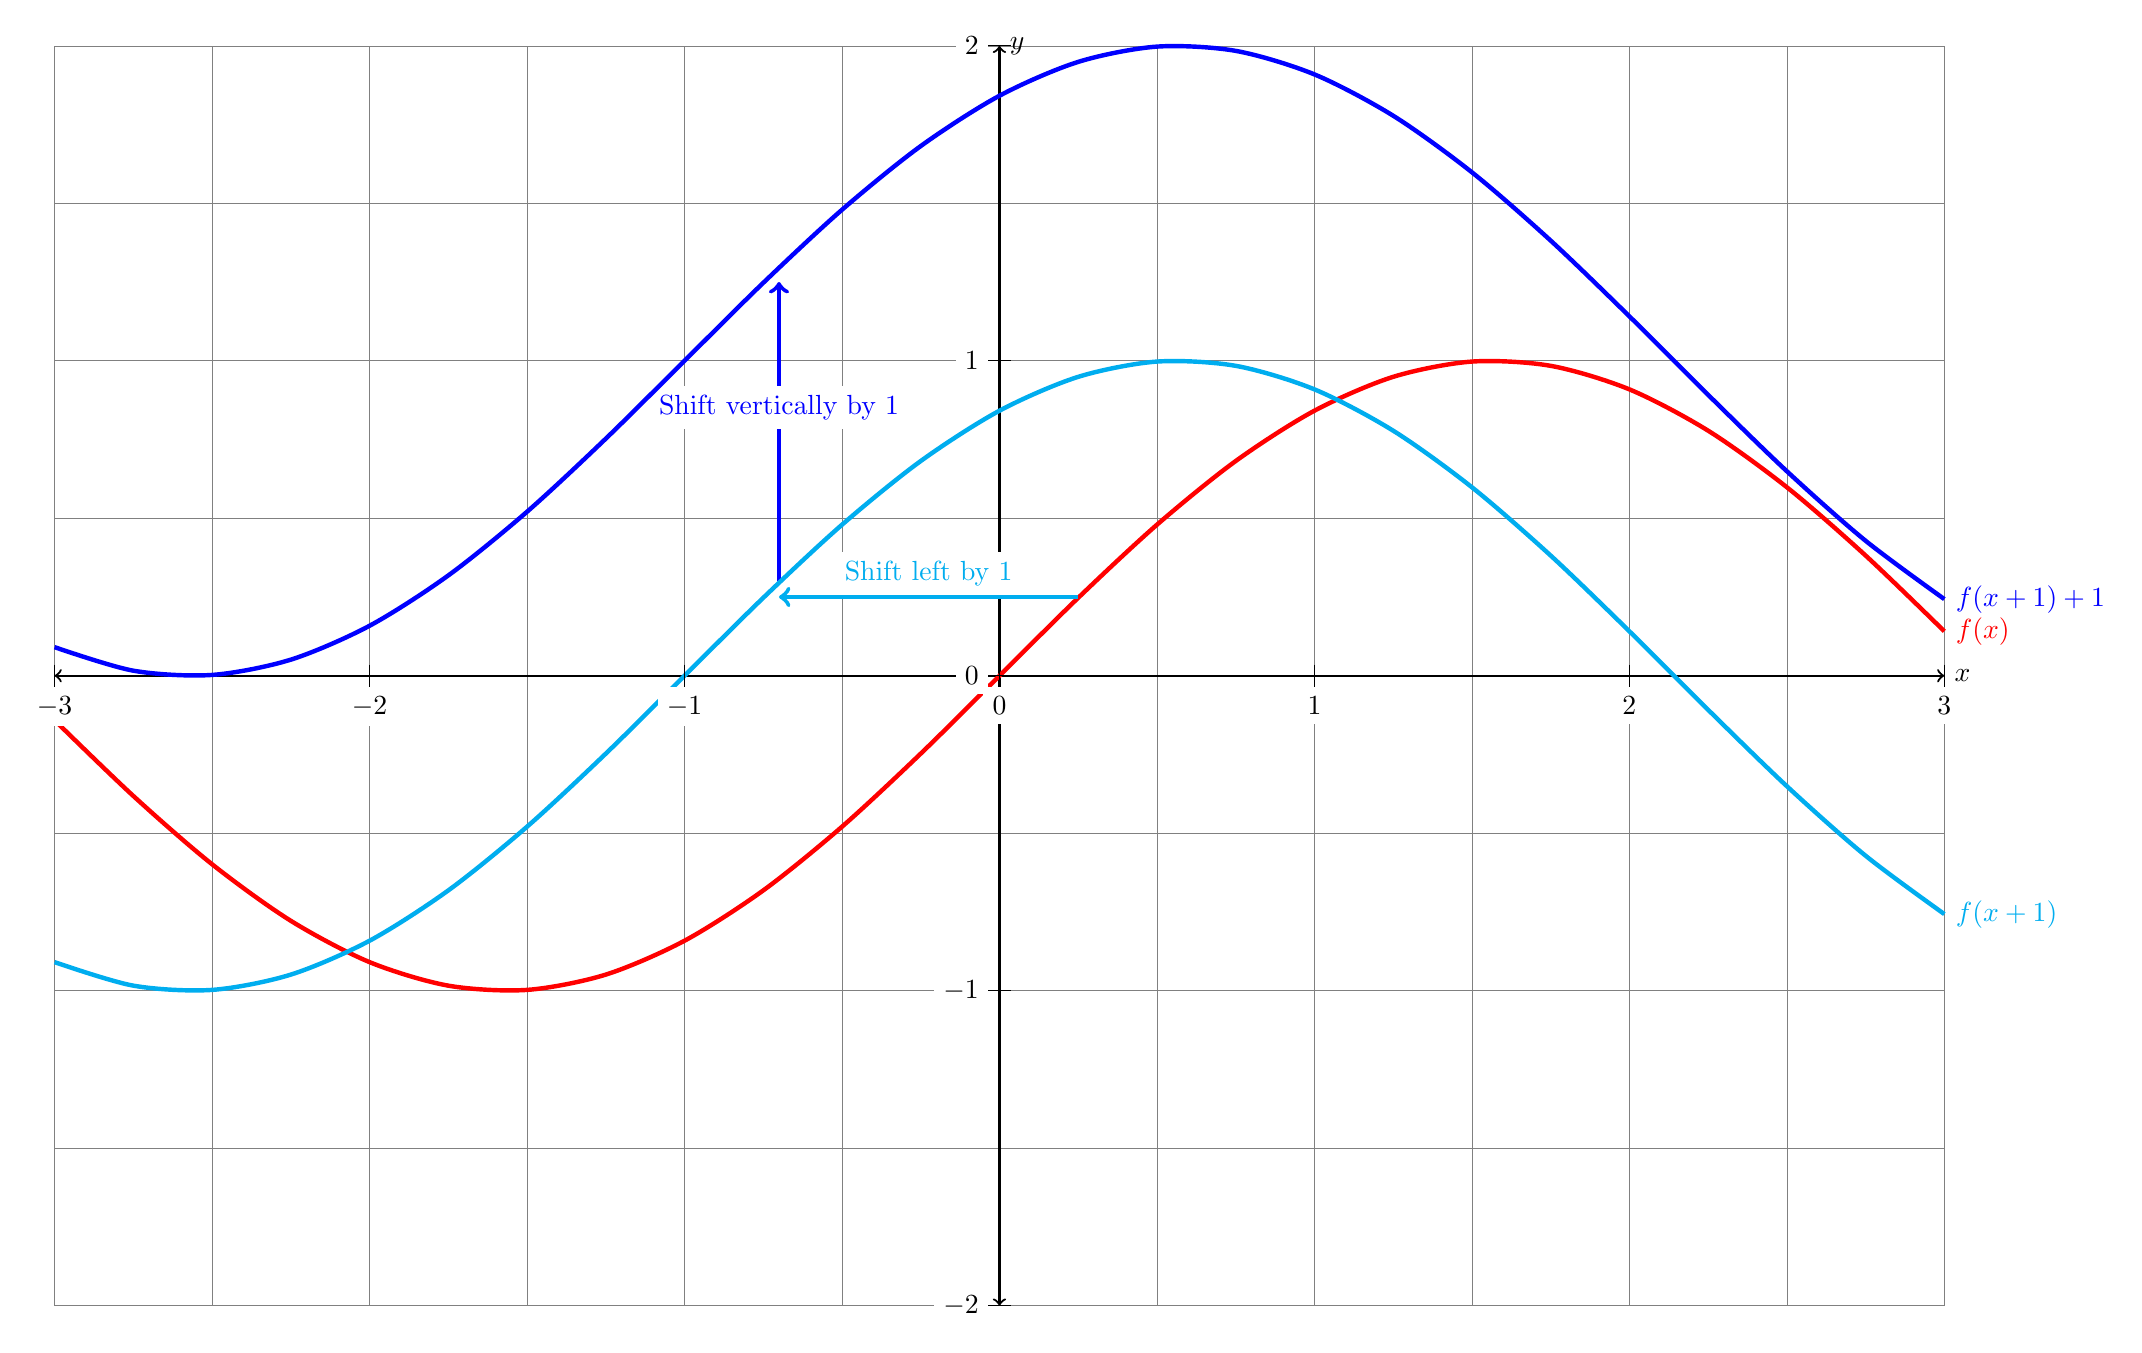
\begin{tikzpicture}[scale=4, mystyle/.style={circle,fill}]

        % setting up the Cartesian Grid. Note "help lines" = "gray, very thin"
        \draw[step=.5cm,help lines] (-3,-2) grid (3,2);
        % setting up the real and imaginary axis. 
        \draw[thick, <->] (-3,0) -- (3,0) coordinate (x axis) node[right] {$x$};
        \draw[thick, <->] (0,-2) -- (0,2) coordinate (y axis) node[right] {$y$};;

	\draw[ultra thick,red,domain=-3:3,smooth] plot (\x,{sin(\x r)}) node[right] {$f(x)$};


	\draw[ultra thick, cyan, ->] (.25,.25) -- (-.70,.25) node[midway, above, fill=white] {Shift left by $1$};
	\draw[ultra thick, blue, ->] (-.70,.30) -- (-.70,1.25) node[midway, above, fill=white] {Shift vertically by $1$};

	\draw[ultra thick,cyan,domain=-3:3,smooth] plot (\x,{sin(\x r + 1 r)}) node[right] {$f(x+1)$};
	\draw[ultra thick,blue,domain=-3:3,smooth] plot (\x,{sin(\x r + 1 r)+1}) node[right] {$f(x+1)+1$};

	\foreach \x in {-3,-2, ..., 3}
		\draw (\x cm,1pt) -- (\x cm,-1pt) node[anchor=north, fill=white] {$\x$};
 	\foreach \y in {-2,-1,0,1,2}
		\draw (1pt,\y cm) -- (-1pt,\y cm) node[anchor=east, fill=white] {$\y$};

	\end{tikzpicture}


\end{document}
